\documentclass[a4paper,14pt]{extarticle}
\usepackage[utf8]{inputenc}
\usepackage[russian]{babel}
\usepackage{graphicx}
\usepackage[top=0.8in, bottom=0.8in, left=0.8in, right=0.8in]{geometry}
\usepackage{pgfplots}
\usepackage{amsmath}
\usepackage{setspace}
\usepackage{titlesec}
\usepackage{float}
\usepackage{chngcntr}
\usepackage{pgfplots}
\usepackage{amsfonts}
\usepackage{pgfplotstable}
\usepackage{multirow}
\usepackage{karnaugh-map}
\usepackage{tikz,xcolor}

\titleformat{\section}[hang]
  {\bfseries}
  {}
  {0em}
  {\hspace{-0.4pt}\large \thesection\hspace{0.6em}}
  
  
\titleformat{\subsection}[hang]
  {\bfseries}
  {}
  {0em}
  {\hspace{-0.4pt}\large \thesubsection\hspace{0.6em}}

%\linespread{1.3} % полуторный интервал
%\renewcommand{\rmdefault}{ftm} % Times New Roman

\newcommand{\nx}{\overline{x}}
\newcommand{\p}{0.31}
\newcommand{\scale}{1.4}

\counterwithin{figure}{section}
\counterwithin{equation}{section}
\counterwithin{table}{section}

\begin{document}
\begin{titlepage}
\centering
Санкт-Петербургский политехнический университет Петра Великого \\
\vspace{0.15cm}
Кафедра компьютерных систем и программных технологий \\
\vspace{6.5cm}

{\centering \textbf{Отчёт по лабораторной работе} \\ 
\vspace{0.15cm}
\textbf{Дисциплина}: Телекоммуникационные технологии \\
\vspace{0.15cm}
\textbf{Тема}: Сигналы телекоммуникационных
систем} \\

\vspace{6.5cm}

\begin{table}[H]
\begin{tabular}{p{\textwidth}@{}r}
{Выполнил студент гр. 33501/4} \hfill {Мальцев  М.С.} \\
{Преподаватель} \hfill {Богач Н.В.} \\
\end{tabular}
\end{table}
\vfill

{\centering Санкт-Петербург \\ 
\vspace{0.15cm}
\today}
\end{titlepage}

\tableofcontents
\newpage

\section{Цель работы}

Познакомиться со средствами генерации и визуализации простых сигналов.

\section{Постановка задачи}

В командном окне MATLAB и в среде Simulink промоделировать синусоидальный и прямоугольный сигналы с различными параметрами. Получить их спектры. Вывести на график.

\section{Теоретический раздел}

\section{Ход работы}

\subsection{Моделирование синусоидального сигнала}

\subsubsection{Получение непрерывного сигнала}

При открытие Simulink был выбран шаблон Simple Simulation.

\begin{figure}[H]
\center{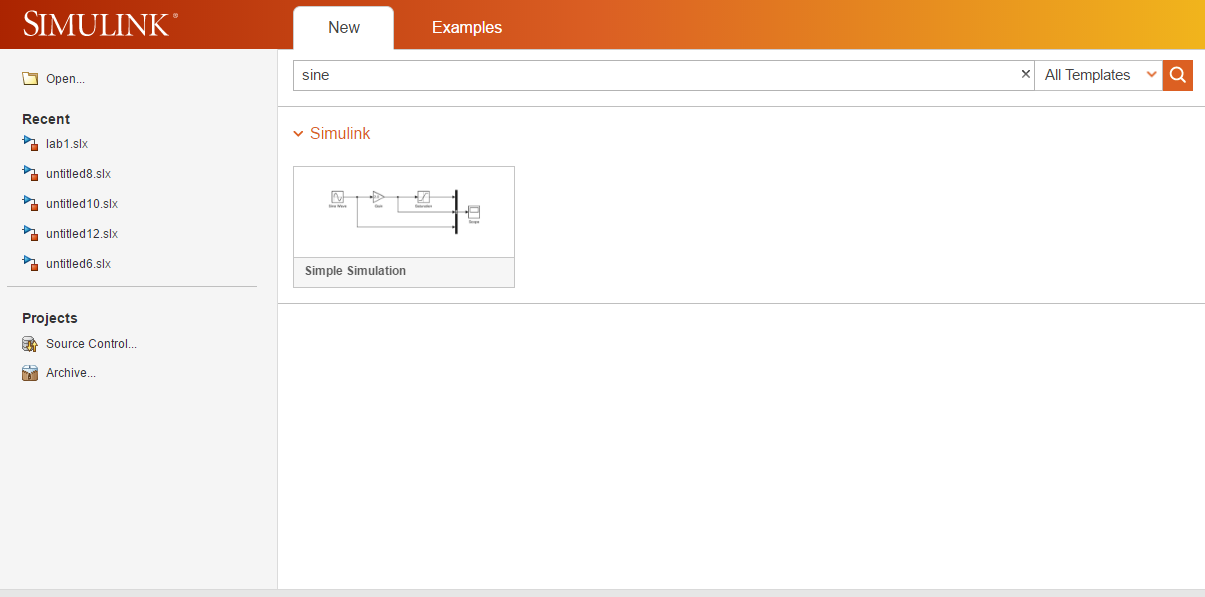
\includegraphics[width=1\linewidth]{img/000.png}}
\caption{Выбор шаблона в начальном окне Simulink.}
\end{figure}

\newpage

Была сгенерирована схема представленная на рисунке \ref{001}.

\begin{figure}[H]
\center{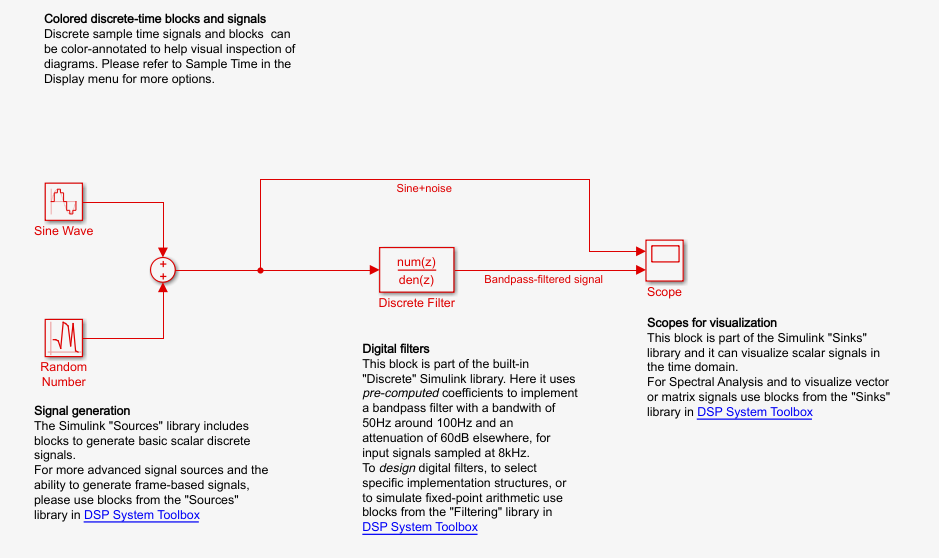
\includegraphics[width=1\linewidth]{img/001.png}}
\caption{Схема автоматически сгенерированная Simulink.}
\label{001}
\end{figure}


Краткое описание назначения элементов:
\begin{itemize}
\item \textbf{Sine Wave} задаёт синусоидальный сигнал с амплитудой 1 и частотой 1 rad/sec
\item \textbf{Gain} усиливает входной сигнал в 2 раза
\item \textbf{Saturation} устанавливает ограничивающие пределы верхний на 0.5 и нижний на -0.5\\
\end{itemize}

Таким образом, при симуляции мы должны увидеть на графике 3 сигнала:
\begin{enumerate}
\item синусоидальный сигнал с амплитудой 1
\item синусоидальный сигнал с амплитудой 2
\item сигнал трапециевидной формы с амплитудой 0.5
\end{enumerate}

Причём, для всех сигналов должен быть одинаковый период,\\ равный 
$\sim$ 6.28 секунды.\\

\newpage

При запуске симуляции получили результаты продемонстрированные на рисунке \ref{002}.

\begin{figure}[H]
\center{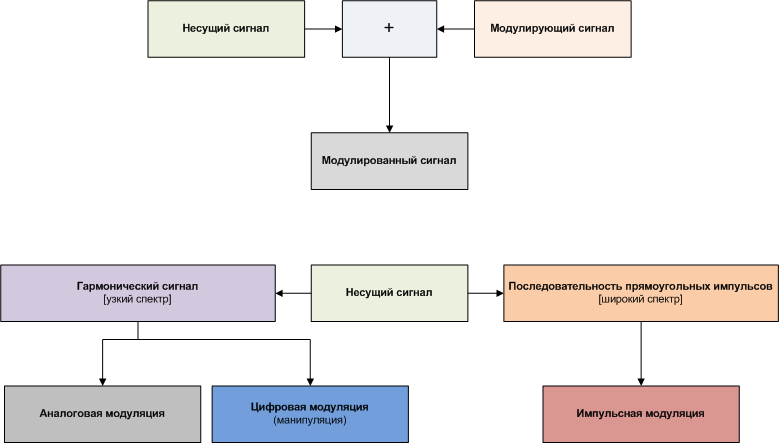
\includegraphics[width=1\linewidth]{img/002.png}}
\caption{Результат симуляция непрерывного сигнала. Окно Scope.}
\label{002}
\end{figure}

Проанализировав результаты симуляции, на соответствие ожиданиям, можно сделать вывод, что она выполнена правильно.

\subsubsection{Получение дискретного сигнала}

Не изменяя общую структуру, представленную на рисунке \ref{001}, изменим для элемента \textbf{Sine Wave} параметр $Sine \ type$ с $Time \ based$ на $Sample \ based$, таким образом мы сделаем сигнал дискретным. Установим $Samples \ per \ period$ на $20\pi$, $\ Sample \ time$ на $0.1$.

\begin{figure}[H]
\center{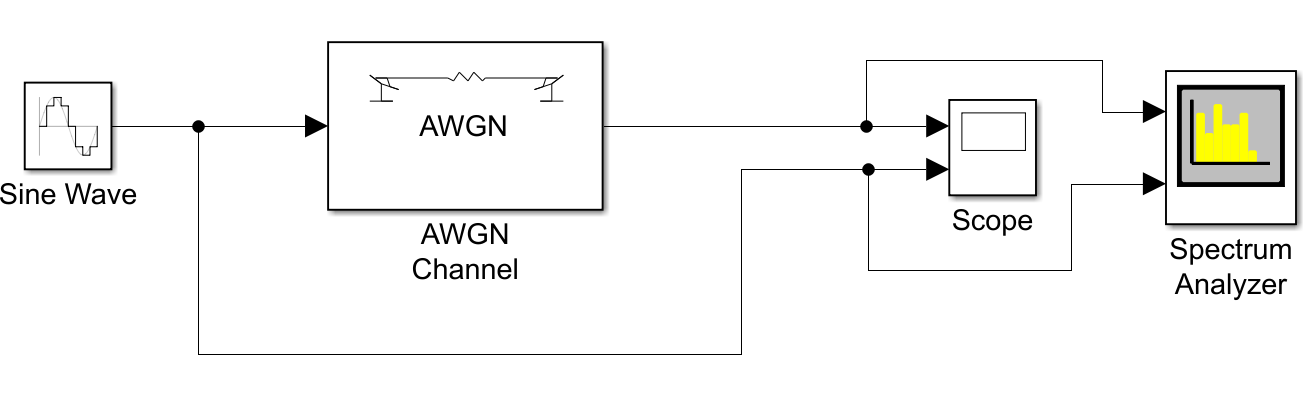
\includegraphics[width=1\linewidth]{img/003.png}}
\caption{Результат симуляция дискретного сигнала. Окно Scope.}
\label{003}
\end{figure}

На рисунке \ref{003} видно, что непрерывный сигнал стал дискретным, что соответствует нашим ожиданиям.

\subsubsection{Получение спектра дискретного сигнала}

Для дискретного сигнала получим его спектр. Для этого установим $Sample \ time$ на 0.01 и $Simulation \ stop \ time$ на 20.

\begin{figure}[H]
\center{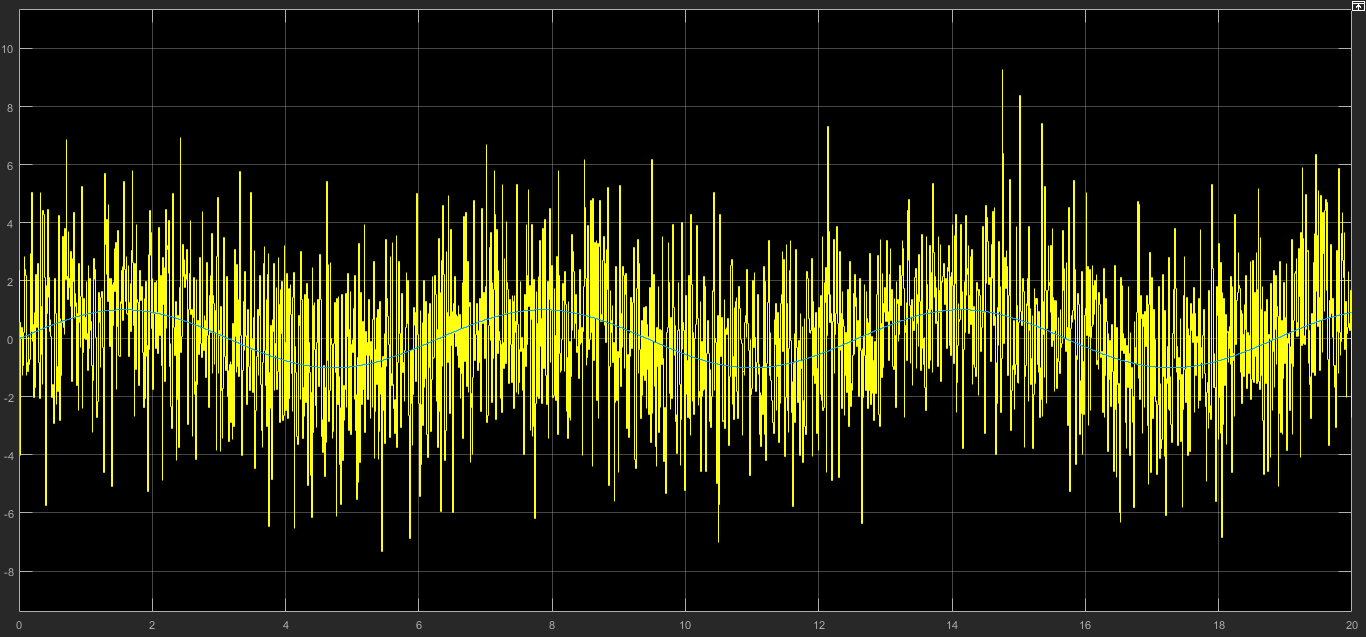
\includegraphics[width=0.65\linewidth]{img/004.png}}
\caption{Схема для исследования спектра дискретного синусоидального сигнала.}
\label{004}
\end{figure}

При запуске симуляции был получен результат, продемонстрированный на рисунке \ref{005}.

\begin{figure}[H]
\center{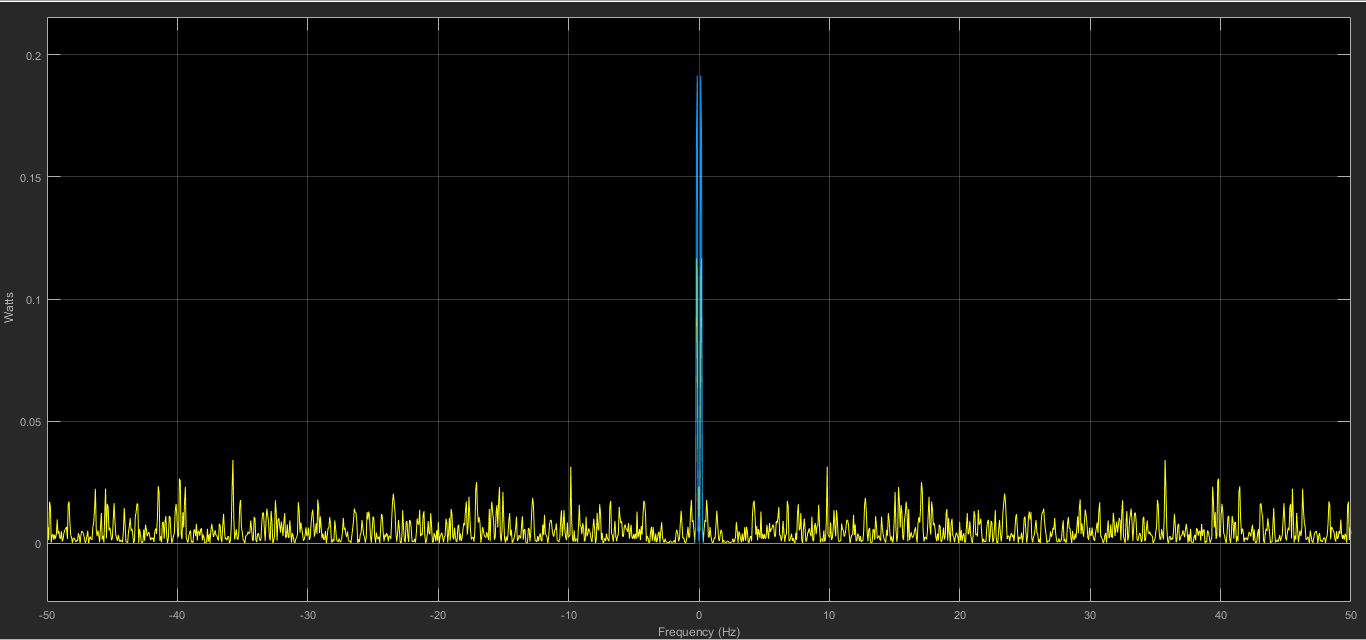
\includegraphics[width=1\linewidth]{img/005.png}}
\caption{Спектр синусоидального дискретного сигнала. Окно Spectrum Analyzer.}
\label{005}
\end{figure}

\newpage

Изменим амплитуду входного сигнала с 1 до 5 и промодулируем снова.

\begin{figure}[H]
\center{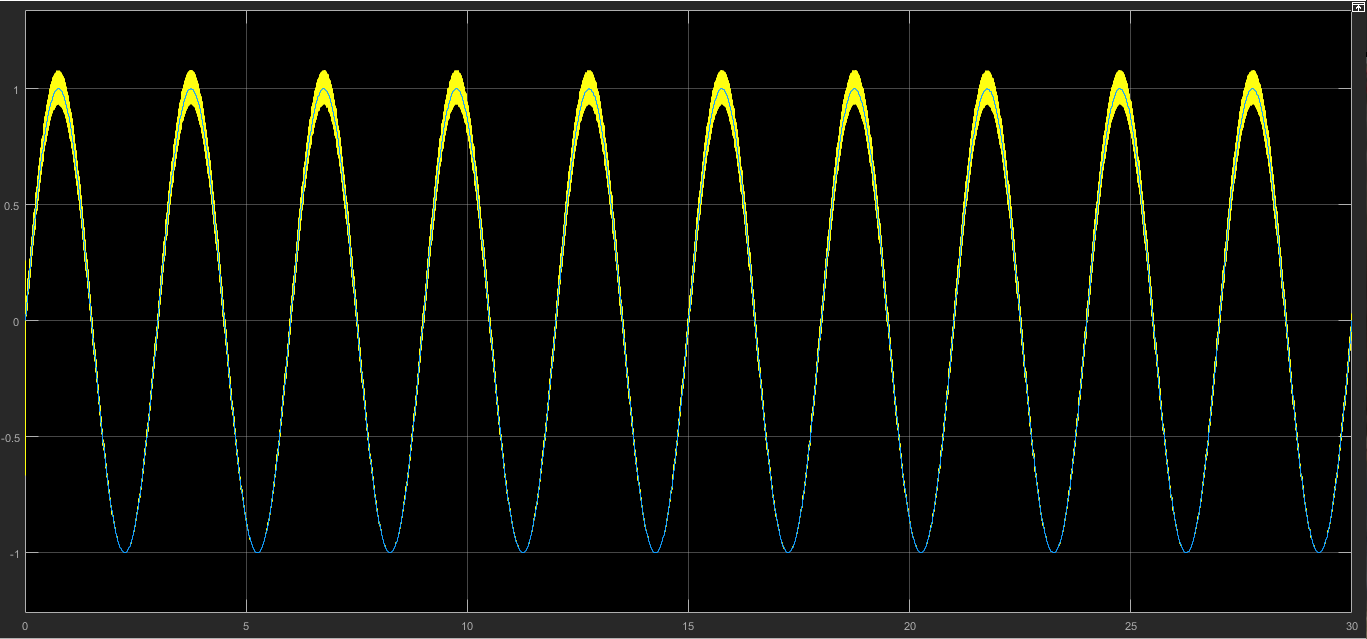
\includegraphics[width=1\linewidth]{img/006.png}}
\caption{Спектр синусоидального дискретного сигнала. Окно Spectrum Analyzer.}
\label{006}
\end{figure}

Изменим $Samples \ per \ period$ c $20\pi$ до $40\pi$

\begin{figure}[H]
\center{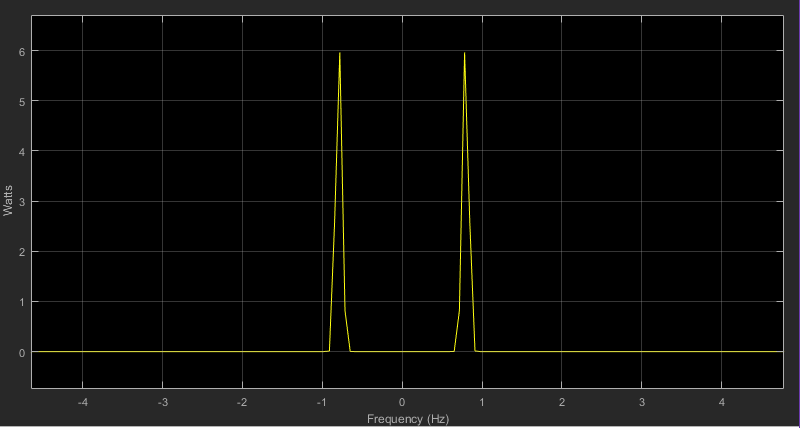
\includegraphics[width=1\linewidth]{img/007.png}}
\caption{Спектр синусоидального дискретного сигнала. Окно Spectrum Analyzer.}
\label{007}
\end{figure}

По полученным результатам варьирования параметров задания сигнала можно сделать вывод о том, что моделирование было проведено верно. На рисунках \ref{005}, \ref{006}, \ref{007} продемонстрировано, что при изменение амплитуды сигнала изменяется амплитуда спектра, причём нелинейно, а при изменение периода обратно пропорционально изменяется частота спектра.

\subsection{Моделирование прямоугольного сигнала}

\subsubsection{Получение дискретного сигнала}

Для исследования прямоугольного дискретного сигнала была введена схема представленная на рисунке \ref{008}. $Simulation \ stop \ time$ установлен на 20.

\begin{figure}[H]
\center{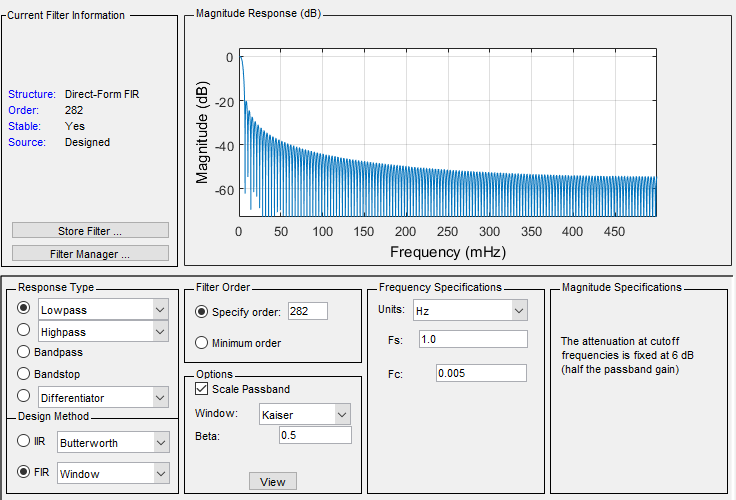
\includegraphics[width=0.6\linewidth]{img/008.png}}
\caption{Схема для исследования прямоугольного дискретного сигнала}
\label{008}
\end{figure}

Для \textbf{Pulse Generator} были заданы параметры представленные на рисунке \ref{009}

\begin{figure}[H]
\center{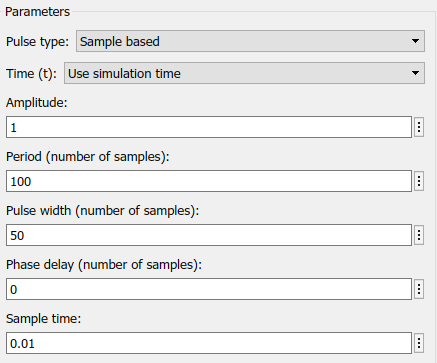
\includegraphics[width=0.6\linewidth]{img/009.png}}
\caption{Окно Block Parameters: Pulse Generator. Раздел Parameters.}
\label{009}
\end{figure}

После моделирования в окне Scope были получены результаты, продемонстрированные на рисунке \ref{010}.

\begin{figure}[H]
\center{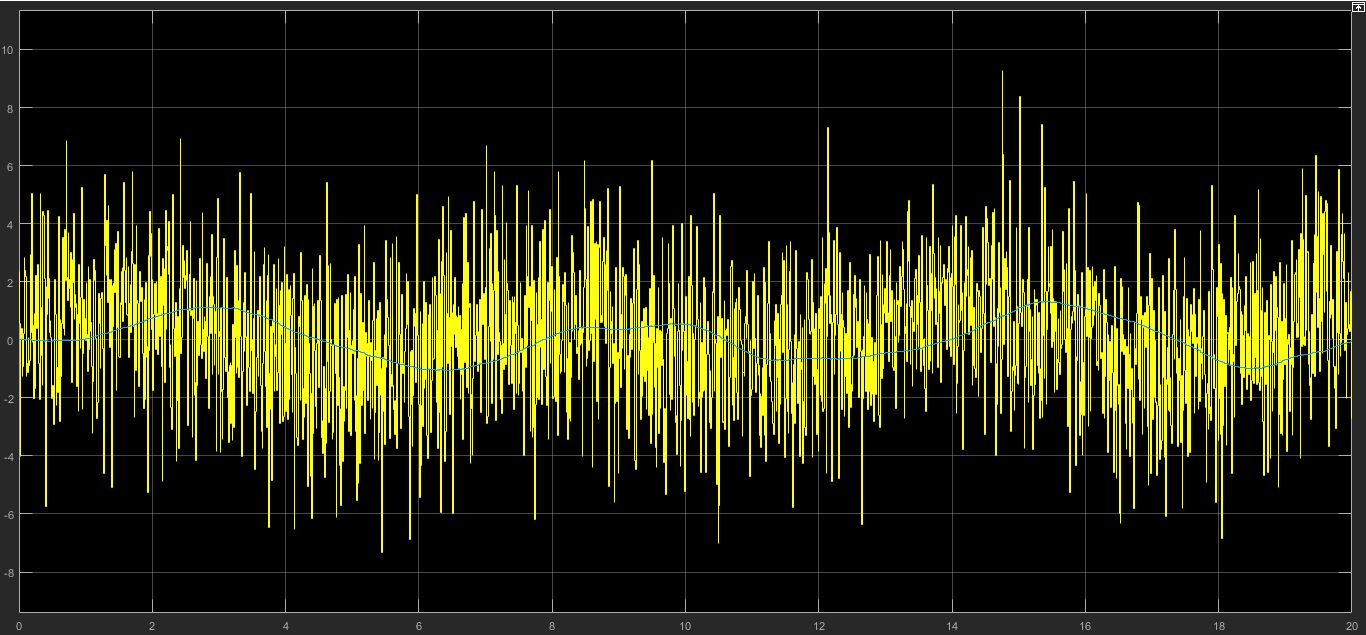
\includegraphics[width=1\linewidth]{img/010.png}}
\caption{Результаты симуляции дискретного прямоугольного сигнала. Окно Scope.}
\label{010}
\end{figure}

По результатам симуляции, визуально можно определить, что поставленная задача, смоделировать прямоугольный сигнал, выполнена.

\subsubsection{Получение спектра дискретного сигнала}

Для получения спектра дискретного сигнала воспользуемся схемой приведённой на рисунке \ref{008}.

Результаты проведённой симуляции приведены на рисунке \ref{011}.

\begin{figure}[H]
\center{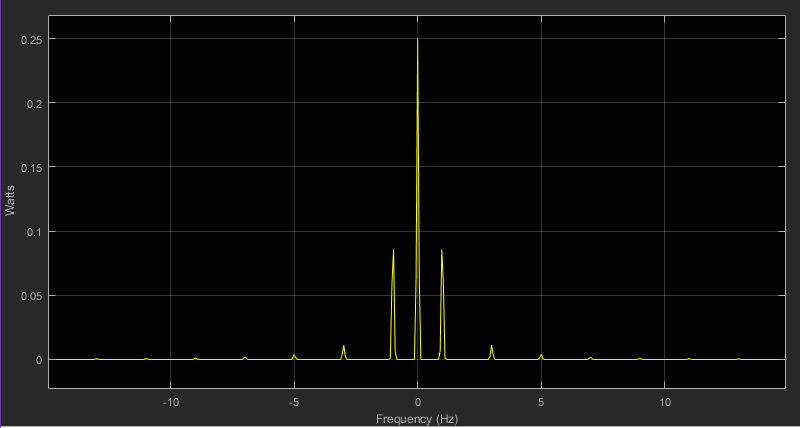
\includegraphics[width=1\linewidth]{img/011.png}}
\caption{Полученный спектр для дискретного прямоугольного сигнала. Окно Spectrum Analyzer.}
\label{011}
\end{figure}

Будем изменять параметры сигнала и следить за изменением спектра.

Изменим период сигнала со 100 до 75.

\begin{figure}[H]
\center{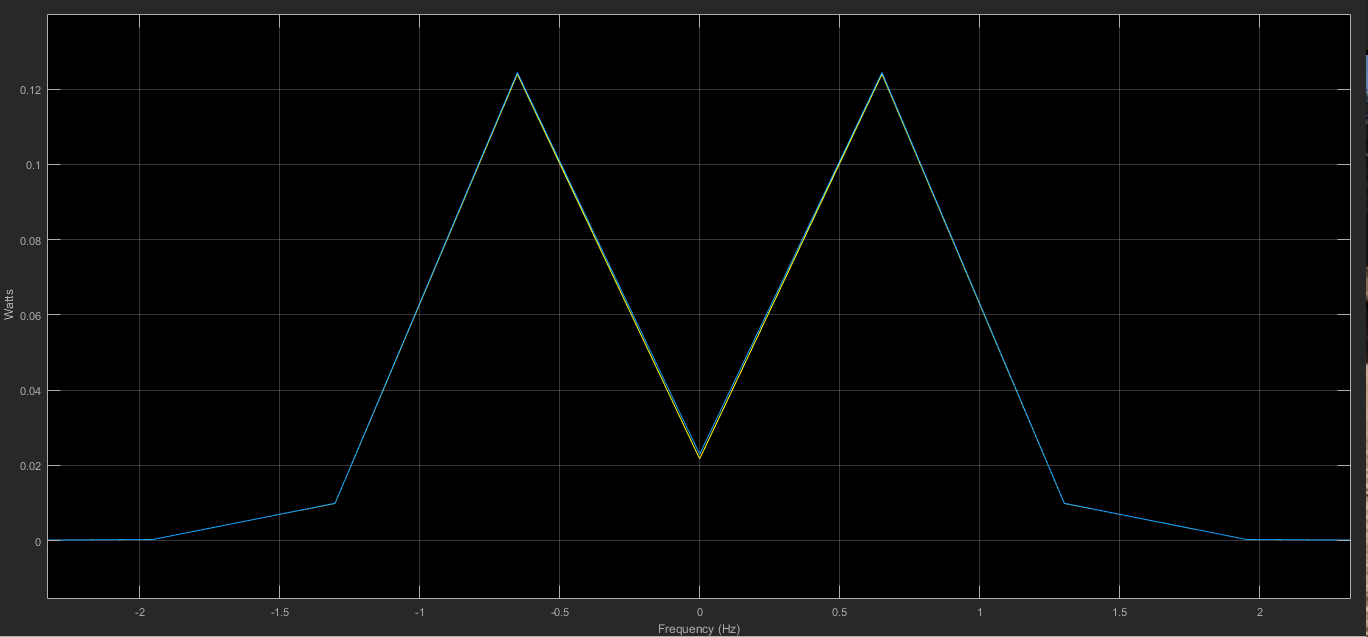
\includegraphics[width=1\linewidth]{img/012.png}}
\caption{Полученный спектр для дискретного прямоугольного сигнала. Окно Spectrum Analyzer.}
\label{012}
\end{figure}

Изменим длину импульса с 50 до 25.

\begin{figure}[H]
\center{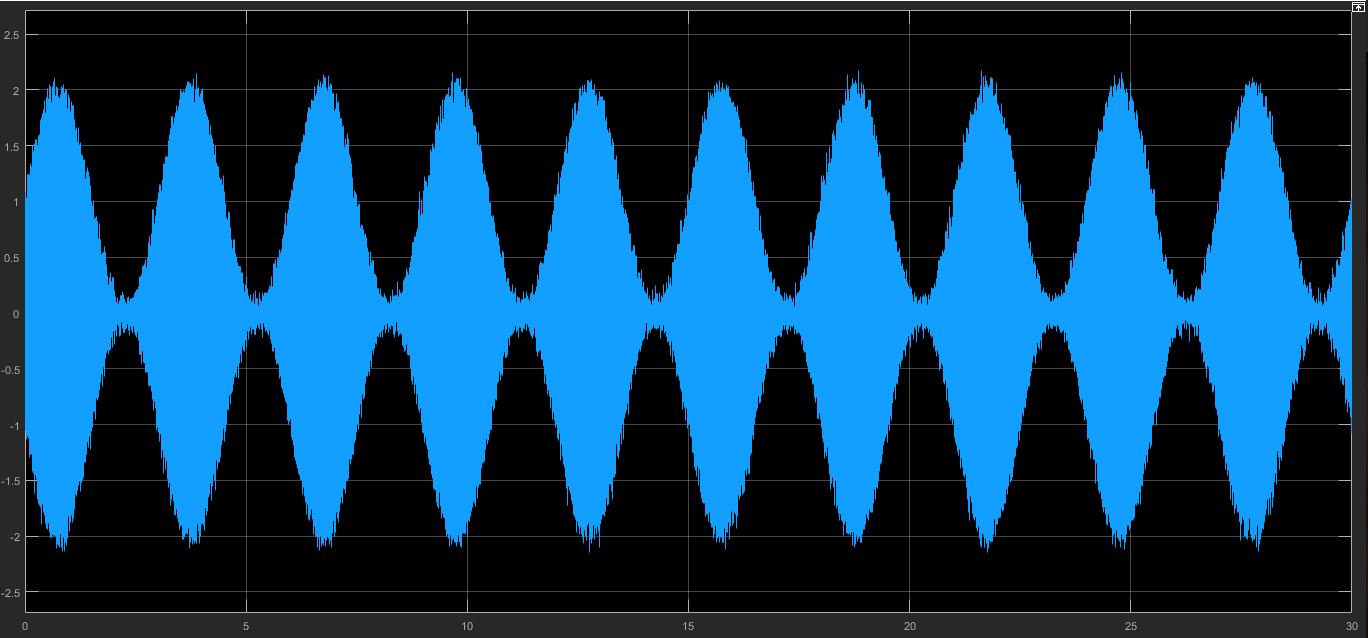
\includegraphics[width=1\linewidth]{img/013.png}}
\caption{Полученный спектр для дискретного прямоугольного сигнала. Окно Spectrum Analyzer.}
\label{013}
\end{figure}

Таким образом, были получены спектры различных дискретных прямоугольных сигналов.

\section{Выводы}

В ходе работы была проведено моделирование различных непрерывных и дискретных сигналов, для дискретных был получен спектр сигнала.

\end{document}
